% Chapter 2

\chapter{Background} % Main chapter title

\label{Chapter2} % For referencing the chapter elsewhere, use \ref{Chapter2}

\lhead{Chapter 2. \emph{Background}} % This is for the header on each page - perhaps a shortened title

%----------------------------------------------------------------------------------------
\section{Introduction}
VANET is a kind of MANET with vehicular node.
Traffic has a great impact on the economy of the 21st century. For the safer and flawless network on the road, we have to use a better protocol and some applications like IDS, IPS.

\section{Related Works}
H. Deng et al.\cite{qa:1} discussed a protocol that requires intermediate nodes for sending RREP message along with the next-hop information. When the source node gets this information,
it sends an RREQ to the next hop to verify that the target node indeed has a route to the intermediate node and the destination. When
the next hop receives a Further Request, it sends a Further
Reply which includes the check result to the source node.
Based on information in Further Reply, the source node judges
the validity of the route. In this protocol, the RREP control
packet is modified to contain the information about next-hop.
After receiving RREP, the source node will again send RREQ
to the node specified as next hop in the received RREP.\\\\

B. Sun et al. \cite{qa:2} use AODV as their routing protocol and
simulation is done in the ns2 simulator. The detection technique
is a neighborhood-based method to detect the black hole
attack and then present a routing recovery protocol to build the
the real path to the destination. Based on the neighbor set
information, a method is improved to deal with the black hole
attack. Source node
sends a modify-Route-Entry (MRE) control packet to the
Destination node to form a correct path by modifying the
routing entries of the intermediate nodes (IM) from source to
destination.\\\\

S. Ramaswamy et al. presented an algorithm in \cite{qa:3} which
claims to prevent the black hole attacks in ad-hoc
network. In this algorithm each node maintains additional data packets, a node must show its honesty. If a node is the
first receiver of an RREP packet, it forwards packets to source
and initiates the judgment process on about replier. The judgment
process depended on the opinion of the network’s nodes about
replier. These neighbors are requested to send their opinion
about a node. When a node collects all opinions of neighbors,
it decides if the replier is a malicious node based on number
rules.\\\\

M.Y. Su \cite{qa:4} proposed the mechanism to detect and separate
malicious nodes, which selectively perform black hole attacks
by deploying IDSs in MANETs (mobile ad hoc networks). All
IDS nodes perform an ABM (Anti-Black hole Mechanism),
which estimates the suspicious value of a node, according to
the amount of abnormal difference between RREQs and
RREPs transmitted from the node. With the prerequisite that
intermediate nodes are forbidden to reply to RREQs if an
intermediate node, which is not the destination and never
broadcasts an RREQ for a specific route, forwards an RREP for
the route, then its suspicious value will be increased by 1 in
the nearby IDS’s SN (suspicious node) table. When the
suspicious value of a node exceeds a threshold, a Block
message is broadcasted by the detected IDS to all nodes on the
network to cooperatively isolate the suspicious node.\\\\

Some attempts have been made for securing wireless monile communication, such as: Secure Efficient Ad hoc Distance vector
routing protocol (SEAD) \cite{qa:5}, the secure on-demand routing
protocol - Ariadne \cite{qa:6}, authenticated routing for ad hoc
networks (ARAN)  \cite{qa:7}, Security-aware ad hoc routing (SAAR)
\cite{qa:8}, Resiliency Oriented Secure (ROS)  \cite{qa:9}, Secure Routing
Protocol (SRP)  \cite{qa:10}, Secure AODV (SAODV)  \cite{qa:11}, Secure Link-
State Protocol (SLSP)  \cite{qa:12}, Cooperative Security-Enforcement
Routing (CSER)  \cite{qa:13}

\section{Research Summary}

A solution is proposed to identify a black hole
node, remove that node from the routing table and finally added to
the blacklist table.
The layout of the network is given below.
%Figure   
\begin{figure}[htbp]
	\centering
	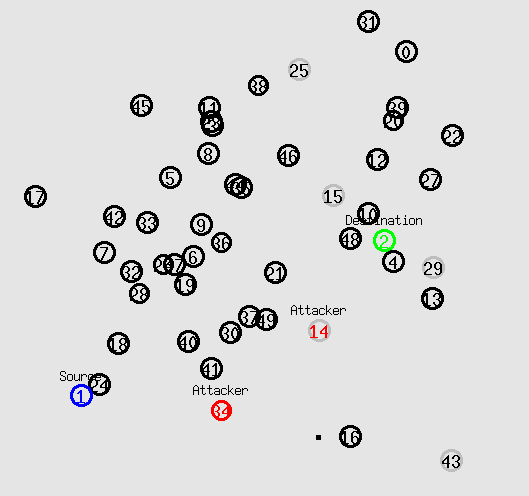
\includegraphics[scale=.5]{black2}
	\rule{35em}{0.5pt}
	\caption[Layout of network]{Layout of Network}
	\label{fig:layout}
\end{figure}


\section{Scope of the Problem}

The purpose of the work is to make a secured network where the blackhole attacker is detected and marked as a malicious node. 50 noded network is used in this study and make 3 of them as malicious. Whenever they drop the packet from a legitimate node. The simulation is run 8 min and Sent total 616 packet \\
To detect the malicious node we had slightly
enhanced the AODV protocol working. In our approach, when
the sender broadcasts the RREQ packet, it will wait for reply.
If the hop count is very short every time then the node is marked as a malicious node.

\section{Challenges}

Vehicular ad-hoc network is a self-composing network with a highly dynamic network topology. For its dynamicity, though
it has many advantages it faces some safety issues. That fall it in threat. If we can fix those issues, VANET can be use
heedlessly.\\
For the Exporting graph from the trace file, there is no much available application. We used a very old software named
tracegraph.\\
Vanet is complex compared to other mobility networks.
